\chapter{2次元共形場理論におけるエンタングルメントエントロピー}\label{chap:EEreview}
この章では2次元共形場理論におけるエンタングルメントエントロピーに焦点をあてて、本研究の内容を説明するために必要な事項を解説する。
\newline

合成系の量子論における基礎的な現象である\textbf{エンタングルメント(entanglement)}は、1935年にEinstein, Podolsky, Rosenによって提案された思考実験\cite{EPR1935}を発端に1982年にAspect, Dalibard, Roger\cite{Aspect1982}らによって実験的に確認され、量子情報理論の分野で理論的に整備されてきた。エンタングルメントやその度合いを定量化する量は様々な分野において様々な文脈で応用・研究されている。例えば量子情報理論においては量子計算や量子誤り訂正を行うための源として応用されたり\cite{HayashietalQI}\cite{nielsen_chuang_2010}、相対論的な場の理論においてはある種の``閉じ込め"が起きて内部の情報にアクセスできなくなった系の熱力学を考える上で重要視されていたり、物性理論においてはトポロジカルな相構造の検出\cite{Kitaev2006}\cite{Levin_2006}や非平衡過程の熱力学的性質を調べるため\cite{Sagawa}\cite{Calabrese_2016}に用いられていたりする。この章では、相対論的な場の理論に焦点を当てて、エンタングルメントの性質を見ていく。

2次元共形場理論は中心電荷$c$によってその性質は大きく変わり、$c<1$のミニマルモデルや$c=1$の自由場は、物性理論での可解格子模型の連続極限にあると考えられているのに対し、$c\gg 1$で重力双対を持つような共形場理論は非常にカオス性の強い理論であると考えられている\cite{Maldacena:2015waa}。そのためエンタングルメントエントロピーの性質も中心電荷によって異なる。特に$c\gg 1$で重力双対を持つような2次元共形場理論でのエンタングルメントエントロピーを相関関数から計算することは難しいが、AdS$_3$/CFT$_2$対応によってAdS$_3$空間での測地線の長さを計算することに対応づけられる。この対応公式は\textbf{笠-高柳公式(Ryu-Takayanagi formula)}\cite{Ryu:2006ef}として知られており、AdS$_3$/CFT$_2$対応やBekenstein-Hawkingエントロピーの面積則への理解につながる公式としてだけでなく、臨界点上の強結合系におけるエンタングルメントの解析にも用いられるなど、様々な応用が考えられている。
\newline

\ref{sec:entanglement},\ref{sec:unruh}節では、エンタングルメントの定義と、場の理論の真空のエンタングルメントの具体例であるUnruh効果を\cite{Ohya}\cite{TakayanagiJapan}\cite{Hotta}\cite{Iso}\cite{Birrell:1982ix}\cite{Crispino:2007eb}\cite{Nishioka:2018khk}を参考にして解説する。\ref{sec:EE},\ref{sec:EEcft2},\ref{sec:RTformula}節では、2次元共形場理論でのエンタングルメントエントロピーの計算方法やその性質を\cite{TakayanagiJapan}\cite{Nishioka:2018khk}\cite{Rangamani:2016dms}\cite{Takayanagi:2012kg}\cite{wu2019ads3}\cite{Calabrese:2004eu}\cite{Calabrese:2009qy}を参考にして解説する。

\section{エンタングルメント}\label{sec:entanglement}
ここでは\ref{sec:unruh}節以降で、場の量子論の状態がもつエンタングルメントを扱う準備として、エンタングルメントの定義を説明する。エンタングルメントは合成系の量子力学で現れる、非局所的な性質をもった現象であり、場の量子論のおいては真空ですらエンタングルメントの構造がある。このことはブラックホールのHawking放射のモデルにおいて本質的な役割を果たし、量子重力理論の性質を調べる上で重要な鍵になると期待されている。

\subsection{有限次元量子力学におけるエンタングルメント}
\subsub{状態}
有限次元複素ヒルベルト空間$\HH=\C^d$で表される量子系の\textbf{状態(state)}、あるいは\textbf{密度行列(density matrix)}$\rho\in M_d(\C)$とは
\begin{align}
\rho \geq 0,\  \rho^\dagger = \rho,\  \tr \rho=1
\end{align}
となる行列のことである。とくに階数$1$の状態$\rho$を\textbf{純粋状態(pure state)}といい、その固有ベクトル$\psi$でノルムが$1$のものをとれば$\rho=\psi\psi^\dagger$と書ける。この$\psi\in\C^d$のことも純粋状態と呼ぶ。純粋状態でない状態を\textbf{混合状態(mixed state)}という。状態全体の集合は凸集合をなし、純粋状態はその端点になっている。したがって混合状態は必ず純粋状態の凸結合に分解できる。
\begin{ex}
	系にハミルトニアン$H\geq 0$が与えられたとき、カノニカル分布$\rho_\beta=e^{-\beta H}/Z(\beta)$は混合状態である。ただし$Z(\beta)=\tr e^{-\beta H}$と書いた。$H$の固有ベクトル$H|i\ra=E_i|i\ra$をとれば、
	\begin{align}
	\rho_\beta=\frac{e^{-\beta H}}{Z(\beta)}=\sum_{i}\frac{e^{-\beta E_i}}{Z(\beta)}|i\ra\la i|
	\end{align}
	となる。これは純粋状態$|i\ra\la i|$の凸結合による$\rho_\beta$の分解になっている。
\end{ex}

\subsub{エンタングル状態}
有限次元複素ヒルベルト空間$\HH_A=\C^m, \HH_B=\C^n (m,n\geq2)$上に記述される系$A,B$に対して、その合成系$A+B$のヒルベルト空間として$\HH=\HH_A\tensor \HH_B=\C^m\tensor \C^n$を考える。ただし$\HH$の内積は$\HH_A,\HH_B$の内積$\la,\ra_A,\la,\ra_B$を用いて、
\begin{align}
\la \psi_A\tensor \psi_B, \phi_A\tensor \phi_B\ra = \la\psi_A,\phi_A\ra_A \la\psi_B,\phi_B\ra_B\ (\psi_A,\phi_A\in \HH_A,\ \psi_B,\phi_B\in \HH_B)
\end{align}
と定めたものを線形拡張して定義する。\footnote{ちなみにヒルベルト空間の直和$\HH_A\directsum \HH_B$は、ベクトル空間としての直和に\[\la \psi_A\tensor \psi_B, \phi_A\tensor \phi_B\ra = \la\psi_A,\phi_A\ra_A +\la\psi_B,\phi_B\ra_B\ (\psi_A,\phi_A\in \HH_A,\ \psi_B,\phi_B\in \HH_B)\]で内積を入れたものである。
}
\begin{oframed}
$\HH_A,\HH_B$の純粋状態$\psi_A,\psi_B$(ノルム$1$のベクトル)のテンソル積$\Psi=\psi_A\tensor\psi_B$はノルム$1$であり、$\HH$の純粋状態となる。このように、$\HH$の純粋状態$\Psi$であって、$\HH_A,\HH_B$のある純粋状態$\psi_A,\psi_B$が存在して$\Psi=\psi_A\tensor\psi_B$と書けるようなものを、\textbf{セパラブル状態(separable state)}という。逆に、$\HH$のセパラブル状態でない純粋状態を\textbf{エンタングル状態(entangled state)}という。
\end{oframed}

$\HH_A,\HH_B$の正規直交基底$\psi_A^i,\psi_B^j$をとれば、Hilbert空間のテンソル積の定義から$\HH$の元を$\Psi=\sum_{i} c_{ij}\psi_A^i \tensor \psi_B^j$と展開できる。展開係数行列$C=(c_{ij})$を極分解して$C=UDV$  ($U,V$はユニタリー行列、$D$は対角行列)と分解できるので、正規直交基底を$\psi_A'=U^T \psi_A, \psi_B'=V\psi_B$と取り換えると、$\Psi=\sum_{i} d_{i}\psi_A^{'i} \tensor \psi_B^{'i}$と、対角的に展開できる。この展開を\textbf{Schmit展開}という。
このとき、展開係数行列$(d_i)$の階数が$1$であることと$\Psi$がセパラブル状態であることは同値である。

\begin{ex}
$\C^2$の基底を$|0\ra, |1\ra$ととると、次の$\HH=\C^2\tensor\C^2$の純粋状態はエンタングル状態である。
\begin{align}
\frac{|0\ra_A|0\ra_B\pm |1\ra_A|1\ra_B}{\sqrt{2}},\ \frac{|0\ra_A|1\ra_B\pm |1\ra_A|0\ra_B}{\sqrt{2}}
\end{align}
特に$(|0\ra_A|0\ra_B+ |1\ra_A|1\ra_B)/\sqrt{2}$は\textbf{EPR(Einstein-Podolsky-Rosen)状態}と呼ばれる。
\end{ex}

\begin{ex}\label{generalentangledstate}
$\HH=\C^d\tensor \C^d$の純粋状態
\begin{align}
|\Psi\ra=\sum_{i=1}^d a_i|i\ra_A |i\ra_B\quad \left(\sum_{i=1}^d a_i^2=1, a_1\neq 0, a_2\neq 0 \right)
\end{align}
はエンタングル状態である。特に$a_1=\cdots=a_d=1/\sqrt{d}$のときの状態を最大エンタングル状態(maximally entangled state)という。
\end{ex}

\begin{ex}
$\HH$上のカノニカル分布$\rho_\beta=e^{-\beta H}/Z(\beta)$に対して、$\HH$を``2倍"したヒルベルト空間$\HH_L\tensor \HH_R,\ \HH=\HH_L=\HH_R$を考え、その上の\textbf{thermofield double状態}を
\begin{oframed}
\begin{align}
\sum_{i} \frac{e^{-\beta E_i/2}}{\sqrt{Z(\beta)}}|i\ra_L |i\ra_R \in \HH_L\tensor\HH_R
\end{align}
\end{oframed}
で定義する。これは上の例\ref{generalentangledstate}のエンタングル状態になっていて、高温極限$\beta=0$のthermofield double状態は最大エンタングル状態に一致する。またこれは混合状態の純粋化の一例にもなっている。また、このように系$\HH$を$2$倍する形式は有限温度の場の理論でも本質的に重要な役割を果たす。
\end{ex}

\subsub{部分トレース}
合成系$\HH=\HH_A\tensor \HH_B=\C^m\tensor\C^n$の混合状態は$End(\C^m\tensor\C^n)=M_m(\C)\tensor M_n(\C)$の元であり、
\begin{align}
\rho=\sum_{i} c_{ij} \rho_A^i \tensor \rho_B^j
\end{align}
と展開できる。

このとき$M_n(\C)$部分のみトレースをとる写像$\tr_B\colon M_m(\C)\tensor M_n(\C)\to M_m(\C)\tensor 1_B$
\begin{align}
\tr_B \rho=\sum_{i} c_{ij}\tr\rho_B^j (\rho_A^i \tensor 1_B)
\end{align}
は$\rho_A^i,\rho_B^j$の展開の仕方によらずに定まり、これを\textbf{部分トレース(partial trace)}という。一般に、セパラブル状態を部分トレースすると純粋状態になり、エンタングル状態を部分トレースすると混合状態になる。

\begin{ex}\label{tfdpartialtrace}
thermofield doule状態の$\HH_R$部分を部分トレースすると
\begin{align}
\tr_R \left(\sum_{i}\frac{e^{-\beta E_i/2}}{\sqrt{Z(\beta)}}|i\ra_L |i\ra_R\right)\left(\sum_{j}\frac{e^{-\beta E_j/2}}{\sqrt{Z(\beta)}}|j\ra_L |j\ra_R\right)^\dagger=\sum_{i}\frac{e^{-\beta E_i}}{Z(\beta)}|i\ra_L\la i|_L\tensor 1_R
\end{align}
となって、$\HH_L$上のカノニカル分布を再現する。
\end{ex}

\subsection{場の量子論におけるエンタングルメントとは}
次に、場の量子論におけるエンタングルメントをどのように定義するかについて解説する。

まず簡単のため、1次元格子系でのエンタングルメントをどのように定義するかを考える。格子間隔$a$をもった有限サイズの1次元格子$\Gamma=\{-aN,-a(N-1),\cdots, -a,0,a,\cdots, a(N-1),aN\}$の各格子点$n\in\Gamma$上に、ヒルベルト空間$\HH_n=\C^d$に記述される自由度が存在しており、各格子間で相互作用している系を考える。たとえば1次元Isingモデルなどがこの例である。

このモデルの状態を記述するヒルベルト空間$\HH$は、各格子点$n\in\Gamma$に乗ったヒルベルト空間$\HH_n$の合成系
\begin{align}
\HH=\tensor_{n\in\Gamma} \HH_n=\tensor_{n\in\Z} \C^d
\end{align}
である。したがって、格子$\Gamma$を2つの部分系$A,B$に分けて$\Z=A\disjointunion B$とすると
\begin{align}
\HH=\left( \tensor_{m\in A} \HH_m \right) \tensor \left( \tensor_{n\in B} \HH_n \right)\coloneqq \HH_A\tensor \HH_B
\end{align}
のように全体系のヒルベルト空間も2つに分解できるので、セパラブル状態やエンタングル状態が定義できる。この系の``連続極限"をとることで、直線$\R$上に定義された$1+1$次元の場の理論において$\R=A\disjointunion B$と系を分解したときに$A$と$B$とのエンタングルメントが定義できると推測できる。

以上の設定は自然に高次元化できる。1次元の場合と同様に、格子理論の``連続極限"をとることで、一般の$\R^d$上の場の理論に対して$\R^d$を2つの領域$A,B$に分けることでエンタングルメントが定義できると推測できる(図\ref{fig:discreteentanglement})。
\begin{figure}[h]
	\centering
	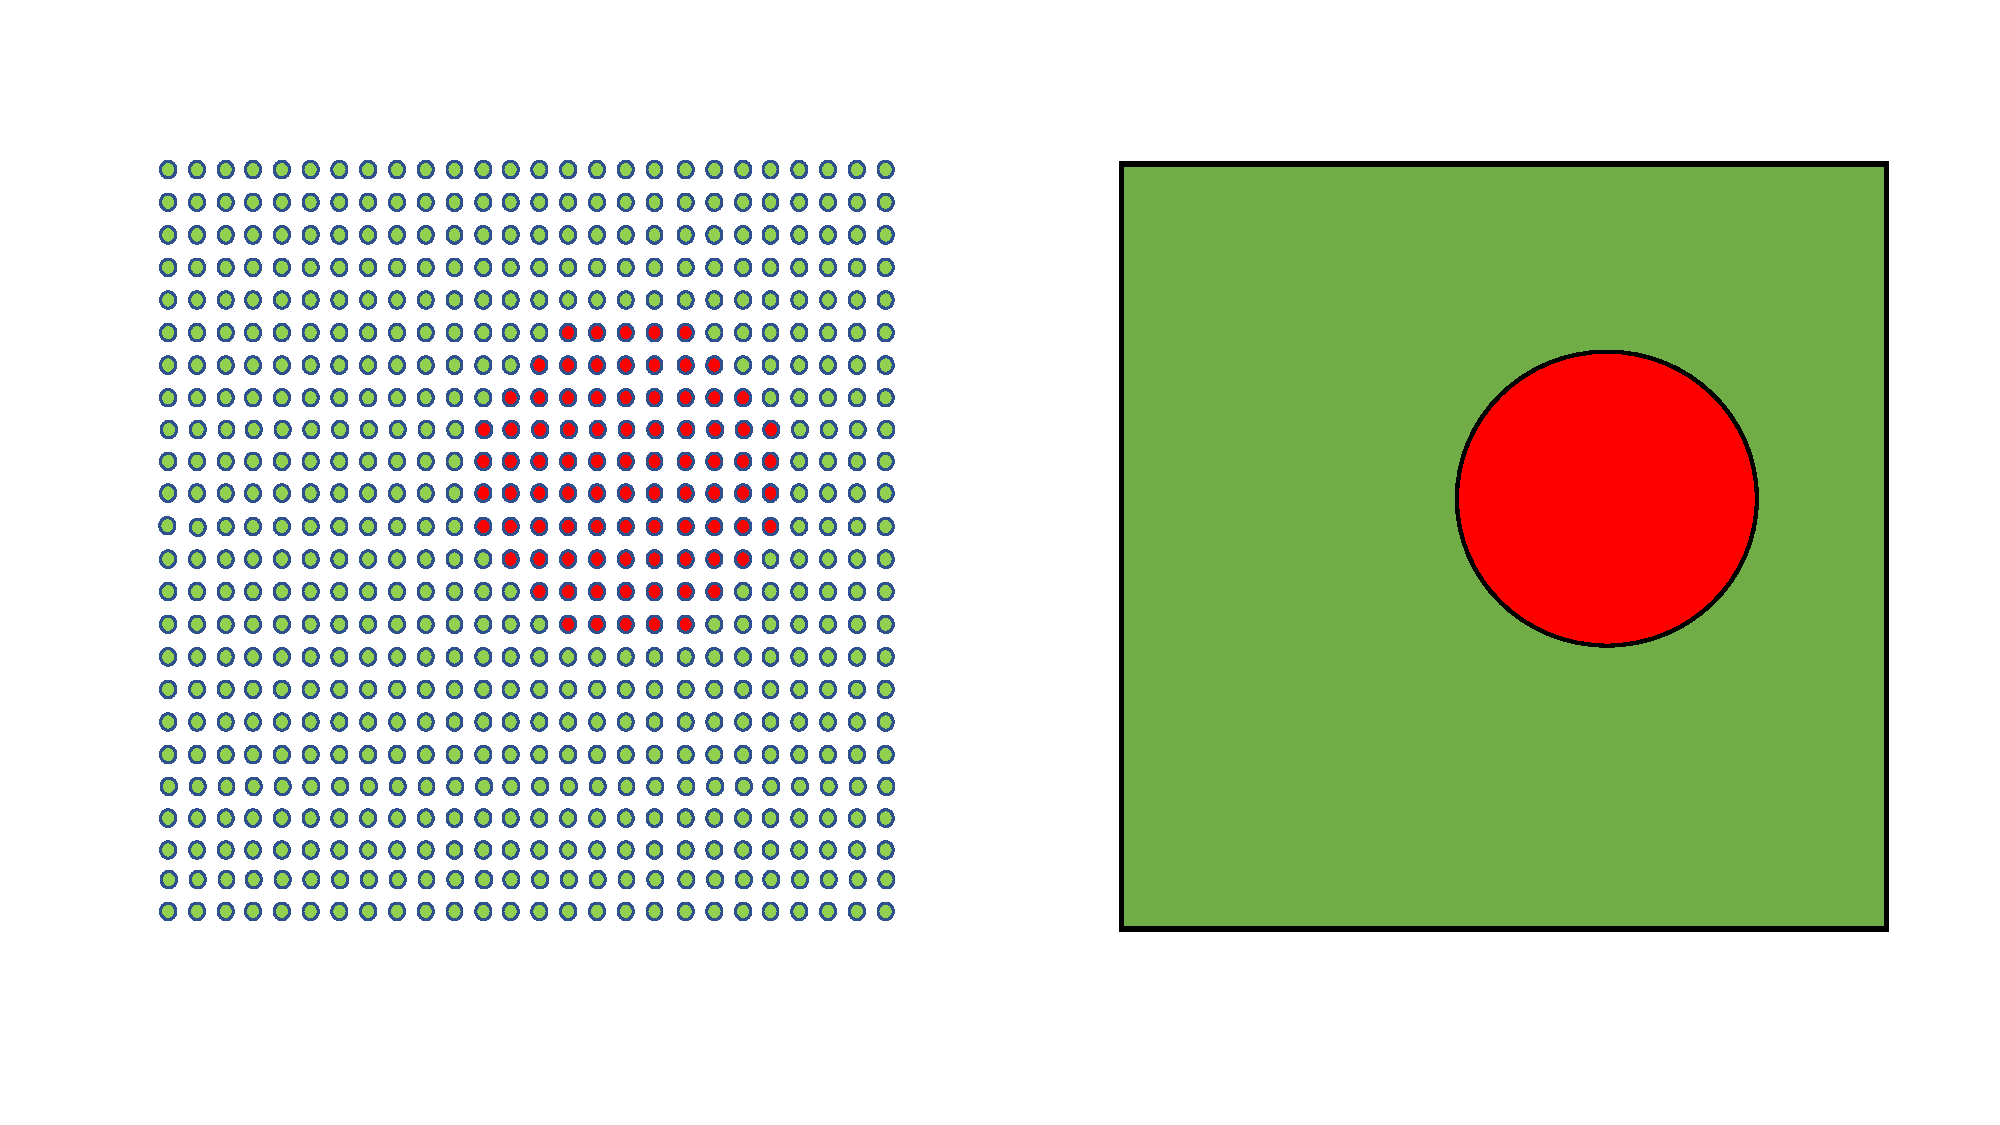
\includegraphics[width=0.7\linewidth]{discreteEntanglement.pdf}
	\caption{左は2次元格子系を表しており、ヒルベルト空間は赤と緑の領域に分解されている。この格子系の``連続極限"をとることで右の連続系でのヒルベルト空間の分解が得られる。}
	\label{fig:discreteentanglement}
\end{figure}

しかし実際に格子理論の領域を$A,B$の2つに分解して、その``連続極限"をとって連続理論へ持っていったときに、連続理論でのヒルベルト空間$\HH_A,\HH_B$やあるいは$A,B$上の局所演算子のなす作用素環$\mathfrak{A}_A,\mathfrak{A}_B$がどのようなものかを具体的に求めることは一般には容易ではない。さらに全系のヒルベルト空間$\HH$ないし局所演算子の作用素環$\mathfrak{A}$を$A,B$のテンソル積で分解できるかどうかも自明ではない。例えばゲージ理論では、$2$つの部分系に分解したときに超選択則による不定性が生じ、格子ゲージ理論ですらエンタングルメントを定義することが難しい\cite{Radicevic:2014kqa}\cite{Casini:2013rba}\cite{Aoki_2017}。こうした連続理論におけるエンタングルメントの問題に対して、代数的(公理論的)場の量子論の立場からアプローチする研究が最近盛んになされている\cite{hollands2018entanglement}\cite{Witten_2018}。

\section{Unruh効果}\label{sec:unruh}
ここでは場の量子論の真空のもつエンタングルメントから生じる現象であるUnruh効果について解説する。Unruh効果はブラックホールのHawking放射のトイモデルとして知られている。また、Unruh効果は代数的(公理論的)場の量子論によって導出できることが知られており、代数的(公理論的)場の量子論の立場からのエンタングルメントへのアプローチの指導原理の一つとなっている。

\subsub{$2$次元共形平坦空間での零質量自由スカラー場の正準量子化}
$1+1$次元Minkowski空間上の零質量自由スカラー場を、$ds^2=-dt^2+dx^2=e^{F(t_c,x_c)}(-dt_c^2+dx_c^2)$となる共形平坦座標$(t_c,x_c),\ (-\infty<t_c<\infty,-\infty<x_c<\infty)$において正準量子化することを考える。Minkowski空間の平坦座標$(t,x)$も自明に共形平坦であり、$(t_c,x_c)$での正準量子化はMinkowski空間の場合とまったく同様に行われる。

いま光円錐座標$x_c^\pm=x_c\pm t_c,\del_{c,\pm}=\frac{1}{2}(\del_{x_c}\pm \del_{t_c})$を導入すれば$ds^2=e^{F(x_c^-,x_c^+)}dx_c^-dx_c^+$で、零質量自由スカラー場の作用は共形不変なので、
\begin{align}
S[X]&=\int d^2 x\sqrt{-\det g} \left(-\frac{1}{2}g^{\mu\nu}\del_\mu X \del_\nu X\right)\notag\\
&=-\frac{1}{2}\int d^2x_c \left( -(\del_{t_c}X)^2+(\del_{x_c}X)^2 \right)\\
&=-\int dx_c^-dx_c^+(\del_{c,-} X \del_{c,+} X)
\end{align}
となる。とくに運動方程式は共形平坦座標においても波動方程式$\del_{c,-}\del_{c,+} X=0$になる。したがって運動方程式の解の完全系として、共形平坦座標での正エネルギーの平面波$e^{ip x_c^-}/\sqrt{2\pi\times 2p}$をとると、正エネルギー解$X$は
\begin{align}
X(x_c^-)=\int_{0}^{\infty} \frac{dp}{\sqrt{4\pi p}} (a_p^{c}e^{ip x_c^-}+a_p^{c\dagger}e^{-ip x_c^-})
\end{align}
と平面波展開できる。また、共形平坦座標におけるハミルトニアン$H_c$は
\begin{align}
H_c=\int_0^\infty dp\  p a_p^{c\dagger} a_p^c
\end{align}
とモード展開できる。

正準同時交換関係を課して$X$を正準量子化すれば、$a_p^{c\dagger},a_p^c$は生成消滅演算子と解釈でき、交換関係
\begin{align}
[a_p^c,a_q^c]=0=[a_p^{c,\dagger},a_q^{c,\dagger}],\quad [a_p^c,a_q^{c,\dagger}]=\delta(p-q)
\end{align}
を満たす。このとき共形平坦座標でのFock真空は$a_p^c|0\ra_c=0$で定義される。

いま$x_c^-$の複素数値関数$f,g$に対してKlein-Gordon双線形形式$(\ ,\ )$を
\begin{align}
(f,g)=-i\int_{-\infty}^\infty dx_c^-  (\overline{f}\del_{c,-}g-(\del_{c,-}\overline{f})g)
\end{align}
で定める。定義より$(f,g)=\overline{(g,f)}$が成り立つことに注意しておく。

正エネルギーの平面波$X_p^c=e^{ip x_c^-}/\sqrt{4\pi p},\ \overline{X_p^c}=e^{-ip x_c^-}/\sqrt{4\pi p}$は、Klein-Gordon双線形形式に対して直交系となす。すなわち$p,q>0$より、
\begin{align}
(X_p^c,X_q^c)&=\delta(p-q)\\ (X_p^c,\overline{X_q^c})&\propto \delta(p+q)=0
\end{align}
となる。

\subsub{Unruh効果}
$1+1$次元Minkowski空間$ds^2=-dt^2+dx^2$の局所座標として、Rindler座標$(t_L,x_L),(t_R,t_R)$を
\begin{align}
t&=\mp a^{-1}e^{ax_{L,R}} \sinh at_{L,R}\\
x&=\mp a^{-1}e^{ax_{L,R}} \cosh at_{L,R}
\end{align}
で定義する。この座標は左右の\textbf{Rindler wedge} $W_L,W_R$上で定義された座標であり、$W_L$と$W_R$は因果的に独立な領域になっている(図\ref{fig:rindlerwedge})。
\begin{align}
W_{L,R}=\{(t,x)\mid x^2>t^2, \mp x>0 \}
\end{align}
\begin{figure}[h]
	\centering
	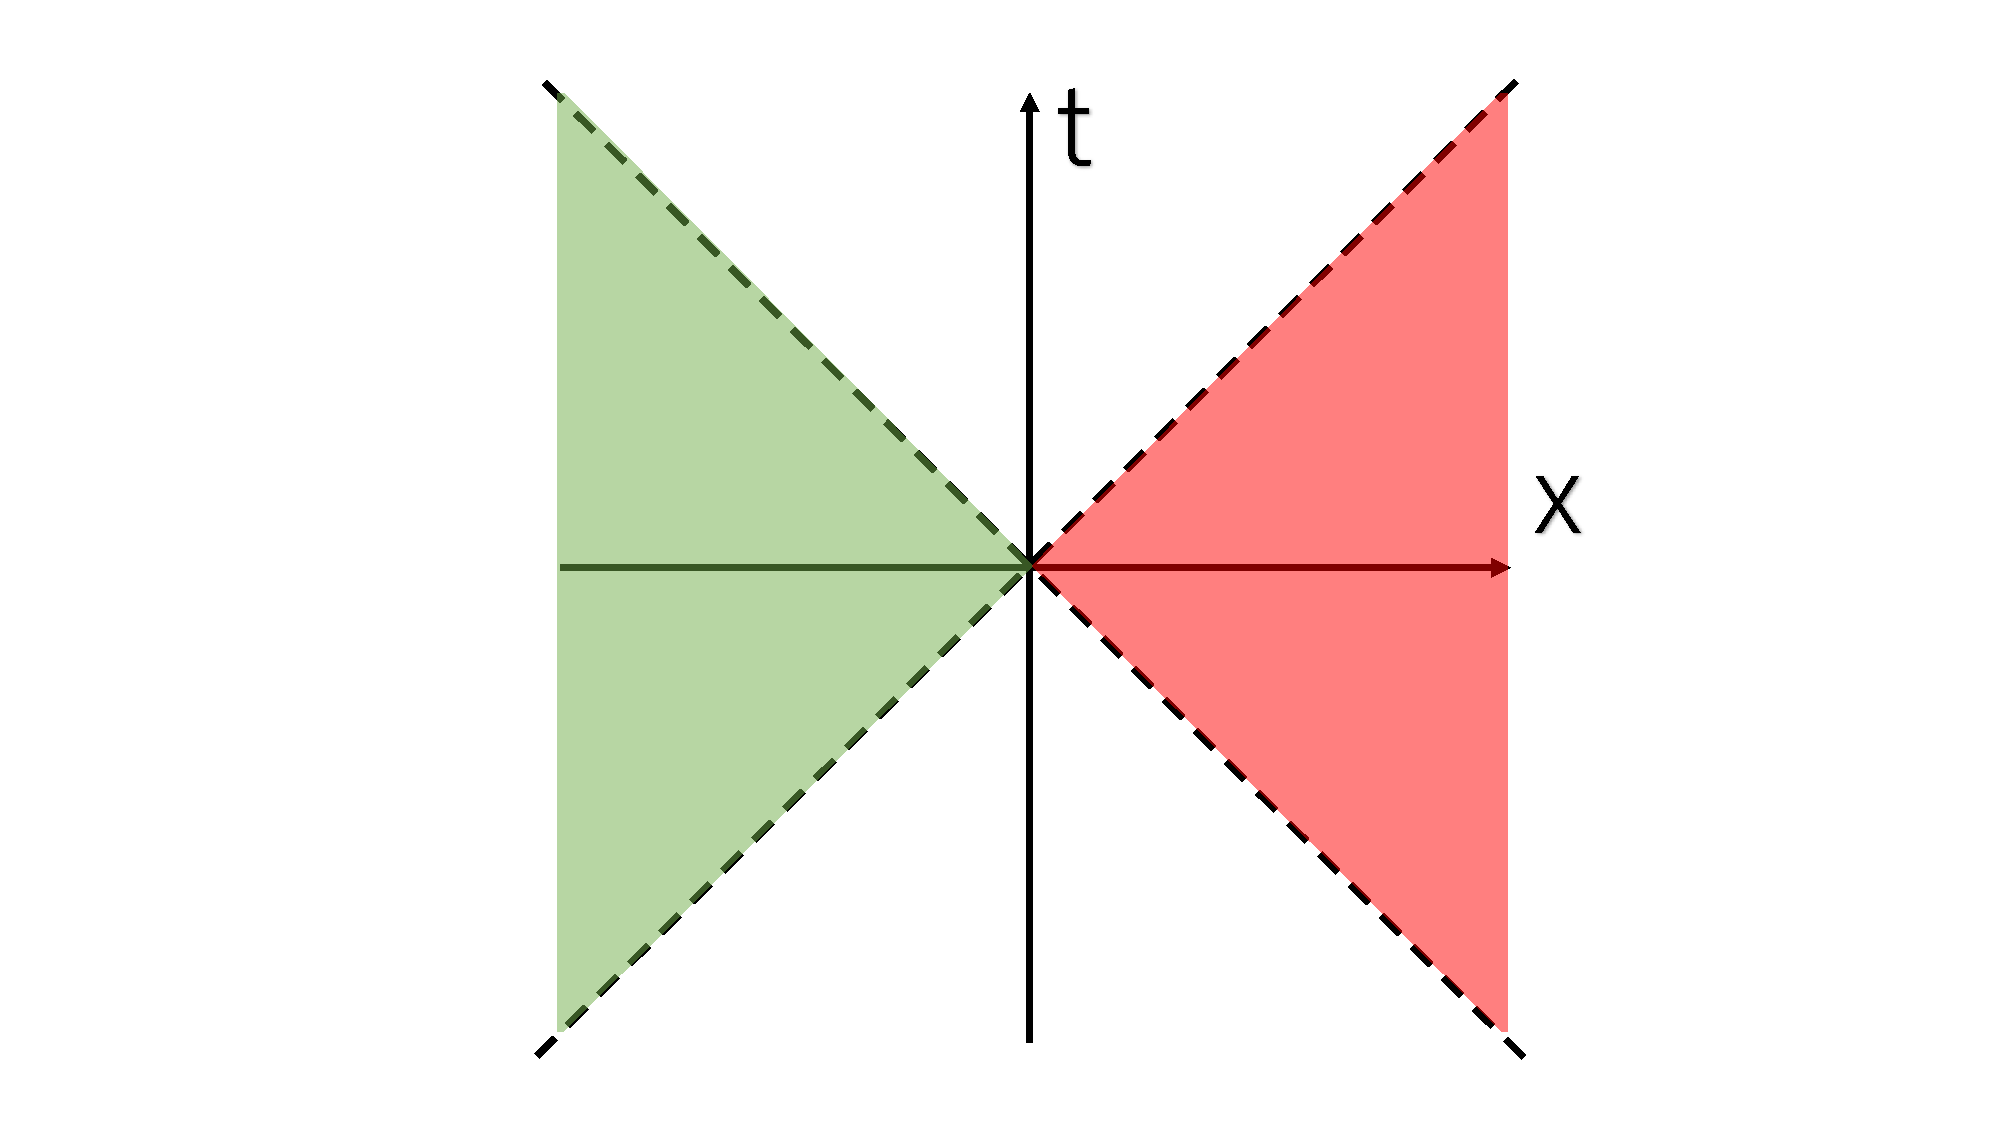
\includegraphics[width=0.7\linewidth]{rindlerwedge.pdf}
	\caption{Minkowski空間に埋め込んだRindler wedgeの図。赤・緑の領域がそれぞれRindler wedge $W_R,W_L$を表している。}
	\label{fig:rindlerwedge}
\end{figure}


計量は$ds^2=e^{2ax_{L,R}}(-dt_{L,R}^2+dx_{L,R}^2)$であるから、$(t_L,x_L),(t_R,t_R)$は共形平坦座標である。時間的Killingベクトル$\del_{t_{L,R}}=a(x\del_t+t\del_x)$に対応するハミルトニアン$K_{L,R}$はLorentzブーストの生成子に他ならず、
\begin{oframed}
\begin{align}
K_{L,R}=\int_{\mp x>0} xT_{00}(t,x) dx\label{modham}
\end{align}
\end{oframed}
と定義する。$K_{L,R}$は$W_{L,R}$の\textbf{モジュラーハミルトニアン(modular Hamiltonian)}とも呼ばれる。

スカラー場$X$の正エネルギー平面波での展開を、Minkowski座標と左右のRindler wedgeの2つで行うと
\begin{align}
X&=\int_{0}^{\infty}\frac{dp}{\sqrt{4\pi p}}(a_p e^{ip x^-}+a_p^{\dagger}e^{-ip x^-})\\
&=\int_{0}^{\infty} \frac{dp}{\sqrt{4\pi p}}(a_p^{L}e^{ip x_L^-}+a_p^{L\dagger}e^{-ip x_L^-}+a_p^{R}e^{ip x_R^-}+a_p^{R\dagger}e^{-ip x_R^-})
\end{align}
と展開され、正準交換関係は
\begin{align}
[a_p,a_q^\dagger]=[a_p^{L},a_q^{L,\dagger}]=[a_p^{R},a_q^{R,\dagger}]=\delta(p-q),\quad  (\text{otherwise})=0
\end{align}
となっている。生成消滅演算子を用いれば、モジュラーハミルトニアンは
\begin{align}
K_{L,R}=\int_{0}^{\infty} dp\  p a_p^{L,R\dagger}a_p^{L,R}
\end{align}
と展開できる。

いま平面波がKlein-Gordon双線形形式に対して直交系になることから、
\begin{align}
a_p=(X_p,X)=\int_{0}^{\infty}dq(a_q^{L}(X_p,X_q^L)+a_p^{L\dagger}(X_p,\overline{X_q^L})+a_p^{R}(X_p,X_q^R)+a_p^{R\dagger}(X_p,\overline{X_q^R}))
\end{align}
と展開できる。Minkowski座標とRindler座標の光円錐座標$x^\pm, x_{L,R}^\pm$は
\begin{align}
x^\pm=-a^{-1}e^{ax_L^\pm}=a^{-1}e^{ax_R^\pm}
\end{align}
で関係づいていることに注意すれば、$X_q^{L,R}=\theta(\mp x^-)\times (\mp ax^-)^{iq/a} /\sqrt{4\pi q}$と書ける。ただし$\theta(x)$は$x>0$で$1$、$x<0$で$0$となるHeaviside関数を表している。

これを用いて展開係数を計算すると
\begin{align}
(X_p,X_q^L)&=\frac{1}{2\pi a}\sqrt{\frac{q}{p}}\left(\frac{a}{p}\right)^{\dfrac{-iq}{a}}\exp\left(\frac{\pi q}{2a}\right)\Gamma\left(\frac{-iq}{a}\right)\\
(X_p,\overline{X_q^L})&=-\frac{1}{2\pi a}\sqrt{\frac{q}{p}}\left(\frac{a}{p}\right)^{\dfrac{iq}{a}}\exp\left(-\frac{\pi q}{2a}\right)\Gamma\left(\frac{iq}{a}\right)\\
(X_p,X_q^R)&=\frac{1}{2\pi a}\sqrt{\frac{q}{p}}\left(\frac{a}{p}\right)^{\dfrac{iq}{a}}\exp\left(\frac{\pi q}{2a}\right)\Gamma\left(\frac{iq}{a}\right)\\
(X_p,\overline{X_q^R})&=-\frac{1}{2\pi a}\sqrt{\frac{q}{p}}\left(\frac{a}{p}\right)^{\dfrac{-iq}{a}}\exp\left(-\frac{\pi q}{2a}\right)\Gamma\left(\frac{-iq}{a}\right)
\end{align}
となり、さらにこれらは
\begin{align}
\int_{0}^{\infty}dq (X_p^R,X_q)(X_q,X_{p'}^L)&=0\\
\int_{0}^{\infty}dq (X_p^R,X_q)(X_q,\overline{X_{p'}^L})&=-\frac{e^{\pi p/a}}{e^{2\pi p/a}-1}\delta(p-p')\\
\int_{0}^{\infty}dq (X_p^R,X_q)(X_q,X_{p'}^R)&=\frac{e^{2\pi p/a}}{e^{2\pi p/a}-1}\delta(p-p')\\
\int_{0}^{\infty}dq (X_p^R,X_q)(X_q,\overline{X_{p'}^R})&=0
\end{align}
を満たしている。$X_p^L$についても同様の式が成り立つ。

したがってMinkowski座標での真空の定義$a_p|0\ra_M=0$から、
\begin{align}
0&=\int_{0}^{\infty} dp (X_q^R,X_p)a_p|0\ra_M=(1-e^{-2\pi q/a})^{-1}(a_q^R-e^{-\pi q/a}a_q^{L\dagger})|0\ra_M\\
&=\int_{0}^{\infty} dp (X_q^L,X_p)a_p|0\ra_M=(1-e^{-2\pi q/a})^{-1}(a_q^L-e^{-\pi q/a}a_q^{R\dagger})|0\ra_M
\end{align}
となるから、Minkowski座標の真空$|0\ra_M$と左右のRindler座標の真空$|0\ra_L,|0\ra_R$は
\begin{align}
|0\ra_M &\propto \exp\left(\int_0^\infty dp\  e^{-\pi p/a}a_p^{L\dagger}a_p^{R\dagger} \right)|0\ra_L\tensor |0\ra_R\\
&=\sum_{n=0}^{\infty}\frac{1}{n!}\int_{p_i>0} dp_1\cdots dp_n e^{-\pi (p_1+\cdots+p_n)/a}a_{p_1}^{L\dagger}\cdots a_{p_n}^{L\dagger}|0\ra_L\tensor a_{p_1}^{R\dagger}\cdots a_{p_n}^{R\dagger}|0\ra_R
\end{align}
と関係していることが分かる。これはthemofield double状態になっていて、実際
\begin{oframed}
\begin{align}
\tr_L|0\ra\la0|_M&\propto\sum_{n=0}^{\infty}\frac{1}{n!}\int_{p_i>0} dp_1\cdots dp_n e^{-2\pi (p_1+\cdots+p_n)/a}a_{p_1}^{R\dagger}\cdots a_{p_n}^{R\dagger}|0\ra_R\la 0|_R a_{p_1}^{R}\cdots a_{p_n}^{R}\\
&=e^{-2\pi a^{-1}K_R}
\end{align}
\end{oframed}
となる。したがってMinkowski空間の真空を右側のRindler空間$W_R$で見ると、逆温度$\beta=2\pi/a$のカノニカル分布に見えることが分かる。この効果を\textbf{Unruh効果(Unruh effect)}\cite{Unruh1976}という。ブラックホールのHawking放射もこれと同様の現象として説明できる。

Unruh効果は、Wightmanの公理系を課した代数的場の量子論の枠組みから導出することもでき、Bisognano-Wichmannの定理\cite{bisognano1975duality}として知られている。これついては\cite{Araki2001}\cite{haag2012local}に詳しい解説が載っている。

\section{エンタングルメントエントロピー}\label{sec:EE}
ここでは純粋状態のエンタングルメントを測る唯一の量であるエンタングルメントエントロピーについて解説する。そして場の量子論の状態のエンタングルメントエントロピーの計算方法であるレプリカ法も説明する。

\subsection{エンタングルメントエントロピーの定義}
\subsub{von Neumannエントロピー}
複素ヒルベルト空間$\HH$上の状態$\rho$の\textbf{(von Neumann)エントロピー}$S(\rho)$を
\begin{oframed}
\begin{align}
S(\rho)=-\tr \rho\log\rho
\end{align}
\end{oframed}
で定める。ただし$-0\log 0=0$としている。

von Neumannエントロピーは正値$S(\rho)\geq 0$で、等号成立は純粋状態のときのみである。また、von Neumannエントロピーはユニタリー変換$U$に対して不変$S(U^\dagger \rho U)=S(\rho)$で、ユニタリーな時間発展で変化しない。

\begin{ex}
カノニカル分布$\rho_\beta=e^{-\beta H}/Z(\beta)$のvon Neumannエントロピーは
\begin{align}
S(\rho_\beta)&=-\tr (e^{-\beta H}/Z(\beta))\log(e^{-\beta H}/Z(\beta))\notag\\
&=\beta \la H\ra_{\rho_\beta}+\log Z(\beta)\notag\\
&=\beta (\la H\ra_{\rho_\beta}-F(\beta))
\end{align}
となる。ただし$\la H\ra_{\rho}=\tr \rho H$は状態$\rho$でのエネルギーの期待値であり、また、$F(\rho)=-\beta^{-1}\log Z(\beta)$はHelmholtz自由エネルギーである。
\end{ex}

\begin{oframed}
合成系$\HH=\HH_A\tensor \HH_B$の状態$\rho$に対して、$B,A$系をトレースアウトしてできる$A,B$系の密度行列を$\rho_A=\tr_B \rho,\ \rho_B=\tr_A \rho$として、$A$の\textbf{エンタングルメントエントロピー(entanglement entropy)}を$S(\rho_A)$で定める。
\end{oframed}

$\rho$が純粋状態なら$S(\rho_A)=S(\rho_B)$となる。実際、$\rho=|\Psi\ra\la\Psi|$で決まるベクトル$\Psi$をSchmit展開すれば
\begin{align}
\Psi=\sum_{i} d_i |\psi_A^i\ra\tensor |\psi_B^i\ra,\ \rho=\sum_{i} d_i^2 |\psi_A^i\ra\la\psi_A^i|\tensor |\psi_B^i\ra\la\psi_B^i|
\end{align}
であり、$\rho_{A}=\sum_{i} d_i^2 |\psi_{A}^i\ra\la\psi_{A}^i|,\rho_{B}=\sum_{i} d_i^2 |\psi_{B}^i\ra\la\psi_{B}^i|$となるので
\begin{align}
S(\rho_A)=-\sum_{i} d_i^2 \log(d_i^2)=S(\rho_B)
\end{align}
が分かる。したがって純粋状態に対しては、部分系への分解の仕方のみでエンタングルメントエントロピーが決まる。$\HH$の混合状態に対しては$S(\rho_A)=S(\rho_B)$が成り立つとは限らない。純粋状態がセパラブルならエンタングルメントエントロピーは$0$であり、エンタングルメントエントロピーは純粋状態のエンタングルメントの強さを測る唯一の量になっている。

例\ref{tfdpartialtrace}より、thermofield double状態のエンタングルメントエントロピーはカノニカル分布のvon Neumannエントロピーに等しい。
\begin{ex}
2次元Minkowski空間上の$t=0$面に零質量自由スカラー場の真空$|0\ra\la 0|_M$を用意する。このときRindler wedge $W_R$のエンタングルメントエントロピーは
\begin{align}
S(\rho_R)&=S(\tr_L |0\ra\la 0|_M)=S(e^{-2\pi a^{-1}K_R}/Z)=2\pi a^{-1}\la K_R \ra_{\rho_R}+\log Z
\end{align}
となる。一般に、場の量子論を2つの空間領域に分解したとき、エンタングルメントエントロピーは真空でさえ0ではなく、しかも紫外発散を含む量になっている。
\end{ex}


\subsub{von Neumannエントロピーの特徴づけ}
複素ヒルベルト空間$\HH$上の密度行列全体の空間$T(\HH)_{1+}$から$[0,\infty]$への写像$\Theta\colon T(\HH)_{1+}\to[0,\infty]$であり、以下の7つの性質を満たすものは定数倍を除いてvon Neumannエントロピ$S$に一致することが知られている。

\begin{enumerate}
\item $\Theta$はユニタリー不変
\begin{align}
\forall U\text{;ユニタリー},\ \Theta(U^\dagger \rho U)=\Theta(\rho)
\end{align}
\item 直和空間$\directsum_{k=1}^n \HH_k$の上の、直和で表される状態$\directsum_{k=1}^n a_k\rho_k,\ \sum_{k}a_k=1$に対して
\begin{align}
\Theta(\directsum_{k=1}^n a_k\rho_k)=\sum_{k=1}^{n}a_k\Theta(\rho_k)+\Theta\left( \text{diag}(a_1,\cdots,a_n) \right)
\end{align}
\item テンソル積空間$\tensor_{k=1}^n \HH_k$の上の、テンソル積で表される状態$\tensor_{k=1}^n \rho_k$に対して、次の\textbf{加法性(additivity)}を満たす。
\begin{align}
\Theta(\tensor_{k=1}^n \rho_k)=\sum_{k=1}^{n}\Theta(\rho_k)
\end{align}
\item テンソル積空間$\HH_1\tensor\HH_2$上の密度行列$\rho_{12}$に対して$\rho_1=\tr_2 \rho_{12},\ \rho_2=\tr_1 \rho_{12}$と書くとき、次の\textbf{劣加法性(subadditivity)}を満たす。
\begin{align}
\Theta(\rho_{12})\leq \Theta(\rho_1)+\Theta(\rho_2)
\end{align}
\item $\dim_\C\HH=1$なら$\Theta(\forall\rho)=0$
\item $\dim_\C\HH<\infty$なら$\Theta(\forall\rho)<\infty$で、$\Theta$は$\rho$の固有値についての連続関数
\item $\dim_\C\HH=\infty$のとき、階数が有限でない密度行列を$\rho=\sum_{n=1}^{\infty} \lambda_n P_n,\ (\lambda_1\geq \lambda_2\geq\cdots\text{かつ}\\n\to \infty\text{で}\lambda_n\to 0)$とスペクトル分解する。このスペクトルにカットオフを入れて定めた$\rho_N=\sum_{n=1}^{N}\lambda_n P_n/\sum_{n=1}^{N}\lambda_n$を定義すると
\begin{align}
\Theta(\rho_N)\to \Theta(\rho)\  (N\to \infty)
\end{align}
と収束する。
\end{enumerate}

\hfill\newline

von Neumannエントロピー(あるいはエンタングルメントエントロピー)はまた、次の不等式を満たすことも知られている。

\textbf{荒木-Lieb不等式}
\begin{align}
|S(\rho_1)-S(\rho_2)|\leq S(\rho_{12})
\end{align}

\textbf{強劣加法性(strong subadditivity)}
\begin{align}
S(\rho_{123})+S(\rho_2)&\leq S(\rho_{12})+S(\rho_{23})\\
S(\rho_{1})+S(\rho_2)&\leq S(\rho_{13})+S(\rho_{23})\label{ssa}
\end{align}

\subsub{Renyiエントロピー}
$\alpha\in(0,1)\union (1,\infty)$に対して、密度行列$\rho$の\textbf{$\alpha-$Renyiエントロピー}を
\begin{oframed}
\begin{align}
S_\alpha(\rho)=\frac{1}{1-\alpha}\log \tr \rho^\alpha
\end{align}
\end{oframed}
で定める。$S(\rho)=\lim_{\alpha\to 1}S_\alpha (\rho)=-\lim_{\alpha\to 1}\del_{\alpha} \log \tr \rho^\alpha$となっている。

\subsection{相対エントロピーとBekenstein bound}
複素ヒルベルト空間$\HH$上の$2$つの状態$\rho,\sigma$の\textbf{相対エントロピー(relative entropy)}$S(\rho||\sigma)$を
\begin{oframed}
\begin{align}
S(\rho||\sigma)=\tr \rho\log(\rho-\sigma)
\end{align}
\end{oframed}
で定める。相対エントロピーは正値$S(\rho||\sigma)\geq 0$で、等号成立は$\rho=\sigma$のときのみである。また、相対エントロピーはユニタリー変換$U$に対して不変$S(U^\dagger\rho U||U^\dagger \sigma U)=S(\rho||\sigma)$で、ユニタリーな時間発展で変化しない。

相対エントロピーはCPTP写像$\Lambda\colon B(\HH)\to B(\HH)$に対して、単調性$S(\Lambda^\ast \rho||\Lambda^\ast \sigma)\leq S(\rho||\sigma)$を満たす。
\begin{ex}
	ある状態$\rho$と逆温度のカノニカル分布$\rho_\beta$の相対エントロピー$S(\rho||\rho_\beta)$は
	\begin{align}
	S(\rho||\rho_\beta)&=\tr \rho\log(\rho-\rho_\beta)\notag\\
	&=-S(\rho)+\beta\la H\ra_{\rho}+\log Z(\beta)\\
	&=\beta(F(\rho)-F(\rho_\beta))
	\end{align}
	と、Helmholtz自由エネルギーの差になる。
\end{ex}

\subsub{CasiniによるBekenstein boundの導出}
ここで、Casini\cite{Casini:2008cr}によるBekenstein boundの導出を紹介する。\textbf{Bekenstein bound}\cite{Bekenstein:1980jp}とは一般的な物理系のもつエントロピーの普遍的な上限を示唆する式のことで、
\begin{align}
S\le O(1)RE
\end{align}
という式である。ただし$S,R,E$は系のエントロピー、典型的な半径、エネルギーを表している。Bekensteinはもともと、ブラックホールに小さな物体を入れた時にブラックホール熱力学の一般化された第二法則を考えて、この不等式を導出した。これに対してCasiniは相対エントロピーを用いて、この不等式を非常に一般的な設定のもとで導出した。

Minkowski空間の零質量自由スカラー場の真空をRindler wedge $W_R$にトレースアウトした密度行列を、モジュラーハミルトニアン$K_R$を用いて$\rho_{\text{vac},R}=e^{-\beta K_R}$と書く。このとき相対エントロピーの正値性から、$W_R$上の任意の密度行列$\rho_R$に対して
\begin{align}\label{bekensteinboundproof}
S(\rho_R)-S(\rho_{\text{vac},R})&=-S(\rho_R||\rho_{\text{vac},R})+\beta(\la K_R \ra_{\rho_R}-\la K_R\ra_{\rho_{\text{vac},R}})\notag\\
&\leq \beta(\la K_R \ra_{\rho_R}-\la K_R\ra_{\rho_{\text{vac},R}})
\end{align}
となる。

モジュラーハミルトニアンはLorentzブーストの生成子であり、\ref{modham}式から$K_A\sim (W_R\text{の``半径''})\times (W_R\text{でのエネルギー期待値})$と評価できる。したがって\ref{bekensteinboundproof}式は、Bekenstein bound $S\leq O(1)\times RE$を与えている。

\subsection{レプリカ法}
$d$次元Minkowski時空上の場の理論をWick回転してEuclid計量にして、$t\to \pm \infty$で系は真空状態にあるという境界条件を置く。$t=\pm \infty$からの経路積分で$t=0$に経路積分によって純粋状態$\rho=|\Psi\ra\la \Psi|$を用意する。

$t=0$の時間一定面での空間領域を$A,B$の$2$つに分けることで、エンタングルメントエントロピーを定義できる。このとき、$\rho$の部分トレースを経路積分として実行して
\begin{oframed}
\begin{align}
\rho_A=\tr_B\rho=\frac{1}{Z_{\R^d}}\int \mathcal{D}\psi_B(\vec{x}\in B)\ \la \psi_B|\Psi\ra\la \Psi|\psi_B\ra
\end{align}
\end{oframed}
とするのが\textbf{レプリカ法(replica trick)}である。

$A$が連結区間$[x_1,x_2]$で、$|\Psi\ra\la\Psi |$が真空状態なら、
\begin{align}
\tr_A \rho_A^n &= \frac{1}{Z^n} \tr_A \left(\int \mathcal{D}\psi_B(\vec{x}\in B)\la \psi_B|\Psi\ra\la |\Psi|\psi_B\ra\right)^n\\
&=\frac{Z_{(\R^d)^n}}{(Z_{\R^d})^n}
\end{align}
となる。ただし$\R^d$上の分配関数を$Z_{\R^d}$と書いた。また、$(\R^d)^n$は$A$を分岐とする$\R^d$の$n$重被覆のことで、$(\R^d)^n$上の分配関数を$Z_{(\R^d)^n}$と書いた。これを図に表すと図\ref{fig:replicatrick}のようになる。
\begin{figure}[h]
	\centering
	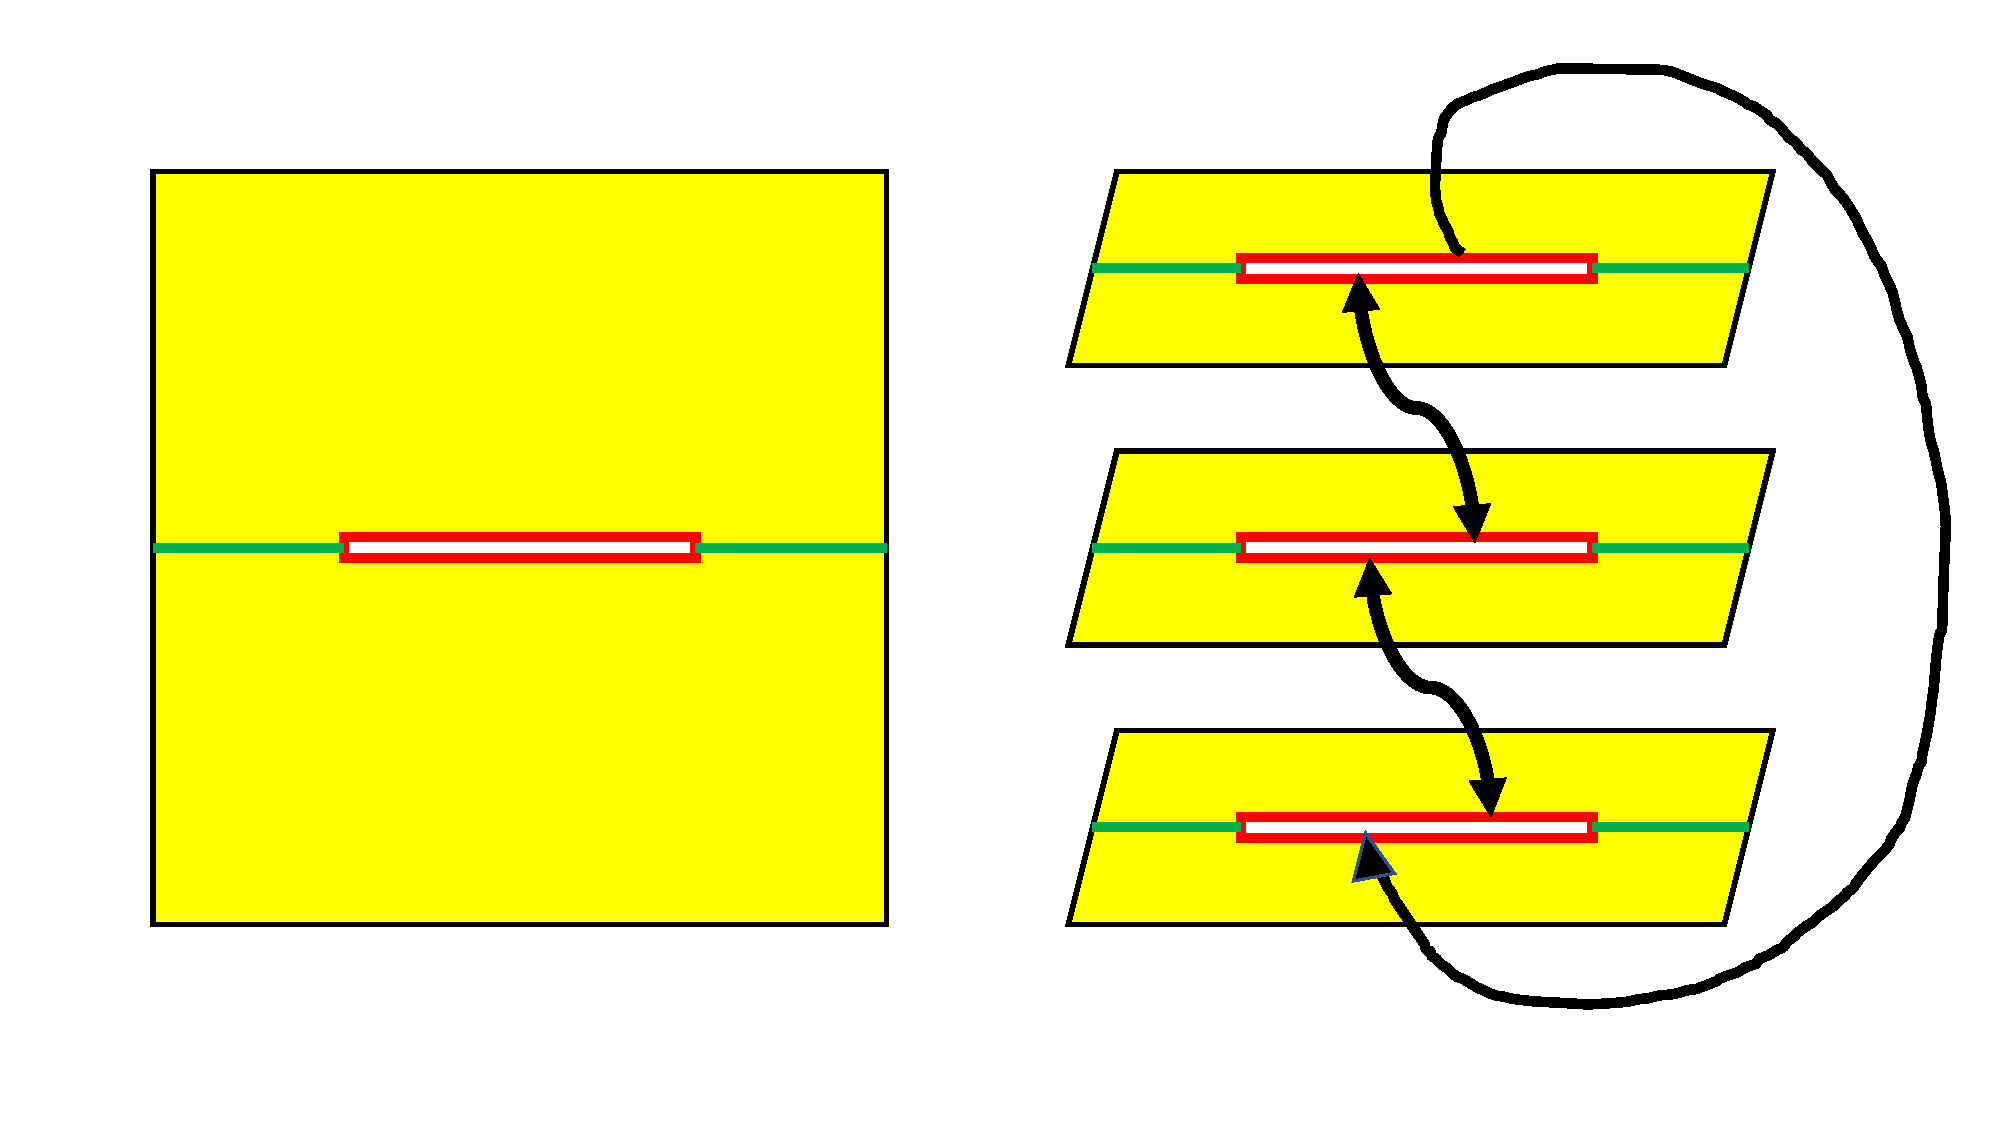
\includegraphics[width=0.7\linewidth]{replicatrick.pdf}
	\caption{左の$\tau=0$に用意された状態$\rho_A$を表している。これを$n=3$倍してトレースをとった$\tr_A\rho_A^3$を表した図が右である。}
	\label{fig:replicatrick}
\end{figure}

したがって真空をトレースアウトしてできた$A$系での混合状態の$n-$Renyiエントロピーは
\begin{align}
S_n(\rho_{A})=-\frac{1}{n-1}(\log Z_{(\R^d)^n} -n \log Z_{\R^d})
\end{align}
である。この$n$を実数へと解析接続して$n\to 1$の極限をとればエンタングルメントエントロピー$S(\rho_A)$が得られる。

\section{2次元共形場理論におけるエンタングルメントエントロピー}\label{sec:EEcft2}
ここでは前節で導入したレプリカ法を用いて、2次元共形場理論におけるエンタングルメントエントロピーを計算する。2次元共形場理論におけるエンタングルメントエントロピーは中心電荷と系の大きさのみで決まり、この結果は格子模型の数値計算によっても確認されている。以下では本研究での解析にも用いた、2次元零質量自由Dirac場の真空のエンタングルメントエントロピーの計算方法を解説し、そのあと一般の2次元共形場理論の真空のエンタングルメントエントロピーの計算方法を解説する。

\subsection{2次元零質量自由ディラック場でのエンタングルメントエントロピー}
\subsub{$A$が直線上の連結区間の場合}
平面$\C$上の2次元零質量自由ディラック場を考え、経路積分によって$\tau=0$の直線上に真空状態を用意する。このとき$\tau=0$の直線を2つの部分系$A,B$に分けてエンタングルメントを定義する。$A$が連結区間$[x_1,x_2]$の場合、レプリカ法を用いて真空$\rho=|0\ra\la 0|$に対して$\tr_A \rho_A^n$を計算するには、$\C$の$n$重orbifoldについての分配関数$Z_{(\C)^n}$を計算すればよい。

これを計算するために、場$\psi,\overline{\psi},\tilde{\psi},\overline{\tilde{\psi}}$をボソン化して得られるスカラー場$X$を用いて、\textbf{ツイスト演算子(twist operator)}
\begin{align}\label{twistopscalarplane}
\sigma_k(z,\overline{z})=e^{i\frac{k}{n}(X_L(z)-X_R(\overline{z}))}=V_{(k/n,-k/n)}(z,\overline{z})\quad \left(k=-\frac{n-1}{2},-\frac{n-3}{2},\cdots \frac{n-1}{2}\right)\\
\overline{\sigma}_k(z,\overline{z})=e^{-i\frac{k}{n}(X_L(z)-X_R(\overline{z}))}=V_{(-k/n,k/n)}(z,\overline{z})\quad \left(k=-\frac{n-1}{2},-\frac{n-3}{2},\cdots \frac{n-1}{2}\right)
\end{align}
を導入する。このとき、場$\psi,\overline{\psi},\tilde{\psi},\overline{\tilde{\psi}}$とツイスト演算子$\sigma,\overline{\sigma}$の演算子積展開は\ref{vertexopOPE}から
\begin{align}
\psi(z)\sigma_k(0,0)&\propto z^{k/n}\\
\tilde{\psi}(\overline{z})\sigma_k(0,0)&\propto \overline{z}^{-k/n}\\
\overline{\psi}(z)\overline{\sigma}_k(0,0)&\propto z^{k/n}\\
\overline{\tilde{\psi}}(\overline{z})\overline{\sigma}_k(0,0)&\propto \overline{z}^{-k/n}
\end{align}
となる。したがって例えば場$\psi$を$z\to e^{2\pi i}z$とツイスト演算子の周りに半時計周りに1周させたときに、$\psi$は位相$e^{2\pi ik/n}$を獲得する。

よって平面$\C$を$n$重にoribifoldした空間での零質量自由Dirac場での相関関数は、平面$\C$にツイスト演算子を挿入した相関関数に等しい。したがって分配関数$Z_{(\C)^n}$は
\begin{align}
\tr_A \rho_A^n&=\frac{Z_{(\C)^n}}{(Z_{\C})^n}\\
&=\prod_{k=0}^{n-1} \la \sigma_k(x_1)\overline{\sigma}_k(x_2) \ra_{\C}\\
&\propto \prod_{k=0}^{n-1}\frac{1}{(x_1-x_2)^{2(h_k+\overline{h}_k)}}
\end{align}
と計算できる。ただし$h_k=\overline{h}_k=k^2/2n^2$である。

$n$が奇数・偶数どちらであっても
\begin{align}
\sum_{k=-(n-1)/2}^{(n-1)/2} \frac{k^2}{n^2} =\frac{1}{12}\left(n-\frac{1}{n}\right)
\end{align}
となる。したがって$\tr_A \rho_A^n \propto (x_1-x_2)^{\frac{1}{6}(n-1/n)}$を得るので、
\begin{align}\label{freediracEEplane}
S(\rho_{A})=\frac{1}{3}\log \frac{|x_1-x_2|}{\epsilon}
\end{align}
となる。ただしここで紫外発散のカットオフパラメーター$\epsilon$を導入した。

\subsub{$A$が円筒上の連結区間の場合}
空間方向が半径$L$の円周にコンパクト化された2次元零質量自由ディラック場の真空のエンタングルメントエントロピーは同様に、$\la \sigma_k(x_1)\overline{\sigma}_k(x_2)\ra_{S_L^1\times \R}$を計算すればよく、
\begin{align}
S(\rho_{A})=\frac{1}{3}\log \left(\frac{2L}{\epsilon}\sin\left(\frac{x_1-x_2}{2L}\right)\right)
\end{align}
となる。

また、直線上の温度$2\pi\beta$のカノニカル分布のエンタングルメントエントロピーは、上のセットアップの座標を$i$倍して、$L$を$\beta$に読み替えればいいので、
\begin{align}
S(\rho_{A})=\frac{1}{3}\log \left(\frac{2\beta}{\epsilon}\sinh\left(\frac{x_1-x_2}{2\beta}\right)\right)
\end{align}
となる。とくに$\beta\to 0$の高温極限($\iff |x_1-x_2|\gg 1$の熱力学極限)をとると、
\begin{align}
S(\rho_{A})\sim\frac{1}{3}\log\frac{2\beta}{\epsilon}+\frac{1}{6}\frac{|x_1-x_2|}{\beta}
\end{align}
となり、第$2$項は通常の熱力学的な示量的エントロピーになっている。

\subsub{$A$が直線上の非連結区間の場合}
平面$\C$の$\tau=0$の直線上の真空について、$N$個の連結成分をもつ区間とそれ以外とのエンタングルメントエントロピーをレプリカ法で計算すると、$n$重にorbifoldされた空間の被覆空間は$g=(n-1)(N-1)$の種数をもったコンパクトRiemann面となる。

とくに$N=2$で$A=[x_1,x_2]\union [x_3,x_4]\ (x_1<x_2<x_3<x_4)$のとき、零質量自由Dirac場でのエンタングルメントエントロピーをレプリカ法で計算すると、各$n$に対して種数$n-1$のコンパクトRiemann面に対する相関関数を計算することになる。したがって$n\geq 2$では、相関関数はモジュライ空間のパラメータの不定性が生じる。しかし最終的に$n\to 1$の極限をとるので、エンタングルメントエントロピーを計算する上ではモジュライパラメータは関係せず、平面上のツイスト演算子$\sigma(x_1)\overline{\sigma}(x_2)\sigma(x_3)\overline{\sigma}(x_4)$の相関関数を計算すればよい。したがって零質量自由Dirac場での$A$のエンタングルメントエントロピーは
\begin{align}
S(\rho_A)=\frac{1}{3}\log\frac{|x_1-x_2||x_3-x_4||x_1-x_4||x_2-x_3|}{\epsilon^2|x_1-x_3||x_2-x_4|}
\end{align}
となる。

\subsection{一般の2次元共形場理論でのエンタングルメントエントロピー}
\subsub{$A$が直線上の連結区間の場合}
平面$\C$上の2次元共形場理論を考え、経路積分によって$\tau=0$の直線上に真空状態を用意する。このとき$\tau=0$の直線を2つの部分系$A,B$に分けてエンタングルメントを定義する。$A$が連結区間$[x_1,x_2]$の場合、レプリカ法を用いて真空$\rho$に対して$\tr_A \rho_A^n$を計算するには、$\C$の$n$重orbifoldについての分配関数$Z_{(\C)^n}$を計算すればよい。

中心電荷$c$をもつ2次元共形場理論で$A=[x_1,x_2]$のときのorbifoldを実現するツイスト演算子は、次のように決まる。

まず共形変換によって平面座標$w$を
\begin{align}
z=\left(\frac{w-x_1}{w-x_2}\right)^{1/n}
\end{align}
によってRiemann球面を$n$等分した領域$z$に移すと、orbifoldによって$z=0,\infty$の2点が特異点になることが分かる。したがってこれに対応して$w=x_1,x_2$にツイスト演算子$\sigma_n,\overline{\sigma}_n$を挿入してorbifoldに対応する位相を獲得させればよい。

共形変換$w\to z$でエネルギー運動量テンソルは非テンソル的な変換をして、$\la T \ra_{w}=0$より、
\begin{align}
\la T \ra_{z}/Z_{(\C)^n}=\frac{c}{24}(1-n^{-2})\frac{(x_2-x_1)^2}{(w-x_1)^2(w-x_2)^2}
\end{align}
となる。これが$w$平面にツイスト演算子$\sigma_n(x_1)\overline{\sigma}_n(x_2)$を挿入したものに等しいとして
\begin{align}
\frac{\la T(w)\sigma_n(x_1)\overline{\sigma}_n(x_2)\ra_{\C}}{\la \sigma_n(x_1)\overline{\sigma}_n(x_2) \ra_{\C}}&\equiv n\la T \ra_{z}/Z_{(\C)^n}\\
&=\frac{c}{24}(n-n^{-1})\frac{(x_2-x_1)^2}{(w-x_1)^2(w-x_2)^2}
\end{align}
とすればよい。

このとき$w\to x_1,x_2$と近づける極限で発散を評価することで$\sigma_n,\overline{\sigma}_n$はそれぞれ
\begin{align}
h=\overline{h}=\frac{c}{24}\left(n-\frac{1}{n}\right)
\end{align}
の共形ウェイトをもつプライマリー場として解釈できることが分かる。

したがって$tr_A \rho_A^n$は
\begin{align}
tr_A \rho_A^n&=\frac{Z_{(\C)^n}}{(Z_{\C})^n}\\
&=\la \sigma_n(x_1)\overline{\sigma}_n(x_2) \ra_{\C}\\
&\propto |x_1-x_2|^{\frac{c}{6}\left(n-1/n\right)}
\end{align}
となるので、エンタングルメントエントロピーは
\begin{oframed}
\begin{align}\label{2dcftplaneEE}
S(\rho_A)=\frac{c}{3}\log\frac{|x_1-x_2|}{\epsilon}
\end{align}
\end{oframed}
となる。平面上の2次元共形場理論での連結区間とそれ以外とのエンタングルメントエントロピーは作用に関わらず中心電荷$c$のみで決まることがわかる。これは、平面上の2次元共形場理論のプライマリー場$2$点関数が定数倍を除いて共形ウェイトのみによって決定できることから来る性質である。

この結果は2次元共形場理論の真空のエンタングルメントエントロピーについての最も基本的な結果であり、1994年にHolzhey,Larsen,Wilczek\cite{Holzhey_1994}によって計算された。

\subsub{$A$が円筒上の連結区間の場合}
空間方向が半径$L$の円周にコンパクト化された2次元共形場理論の真空のエンタングルメントエントロピーを考える。円筒は平面$\C-\{0\}$から共形変換
\begin{align}
w=\tan\left(\frac{\pi z}{L}\right)
\end{align}
によって移すことができるので、ツイスト演算子がプライマリー場であることから、
\begin{oframed}
\begin{align}\label{2dcftcylEE}
S(\rho_A)=\frac{c}{3}\log \left(\frac{2L}{\epsilon}\sin\left(\frac{x_1-x_2}{2L}\right)\right)
\end{align}
\end{oframed}
となる\cite{Calabrese:2004eu}。

同様に平面上の温度$2\pi\beta$のカノニカル分布のエンタングルメントエントロピーは、上の設定を$i$倍して
\begin{oframed}
\begin{align}\label{2dcftthermalEE}
S(\rho_{A})=\frac{c}{3}\log \left(\frac{2\beta}{\epsilon}\sinh\left(\frac{x_1-x_2}{2\beta}\right)\right)
\end{align}
\end{oframed}
となる。とくにとくに$\beta\to 0$の高温極限($\iff |x_1-x_2|\gg 1$の熱力学極限)をとると、
\begin{align}
S(\rho_{A})\sim\frac{c}{3}\log\frac{2\beta}{\epsilon}+\frac{c}{6}\frac{|x_1-x_2|}{\beta}
\end{align}
となり、第$2$項は通常の熱力学的な示量的エントロピーになっている。

\subsub{$A$が非連結区間の場合}
$A$が2つの連結成分からなる非連結区間$A=[x_1,x_2]\union [x_3,x_4]\ (x_1<x_2<x_3<x_4)$の場合、零質量自由Dirac場のときと同様に$n\to 1$の極限を考えることで平面の4点関数を計算すればいい。しかし一般の共形場理論では複比の部分の不定性を決定できず、一般には
\begin{align}
S(\rho_A)=\frac{c}{3}\log\frac{|x_1-x_2||x_3-x_4||x_1-x_4||x_2-x_3|}{\epsilon^2|x_1-x_3||x_2-x_4|}+(\text{複比から来る項})
\end{align}
という形になる。

\section{AdS$_3$/CFT$_2$対応についての笠-高柳公式}\label{sec:RTformula}
ここではAdS$_3$/CFT$_2$対応についての笠-高柳公式を解説する。この公式は、\ref{chap:adscftreview}章で解説したAdS$_3$/CFT$_2$対応を用いて、重力双対を持つような2次元共形場理論でのエンタングルメントエントロピーをAdS$_3$空間内の測地線の長さに関係づける公式である。後に見るように、笠-高柳公式はある意味でBekenstein-Hawking公式の拡張になっており、AdS/CFT対応やブラックホール物理と量子情報理論を関係づける公式としてさまざまな応用研究がなされている。

\subsection{笠-高柳公式}
\subsub{公式}
\textbf{笠-高柳公式(Ryu-Takayanagi formula)}は、重力双対をもつような2次元共形場理論での部分系$A$についてのエンタングルメントエントロピー$S_A$に対して、次の対応を主張する。
\begin{oframed}
\begin{align}
S_A = \min_{\substack{\del\gamma=\del A\\ \gamma\text{と}A\text{で作られるループは0にホモロガス}}} \frac{\text{length}(\gamma)}{4G}
\end{align}
\end{oframed}
ここで、$\gamma$は$A$の境界からAdS$_3$の内部へ伸びる曲線である。条件「$\del\gamma=\del A$」によって曲線$\gamma$と部分系$A$の境界が一致していることが要請されている。また、「min」をとることから曲線$\gamma$は測地線になることも要請される。また、2つ目の条件「$\gamma$と$A$で作られるループは0にホモロガス」はホモロジー条件(homology constraint)と呼ばれ、$\gamma$と$A$で作られるループが穴を囲まないことを要請している。

笠-高柳公式はLewkowycz,Maldacena\cite{Lewkowycz:2013nqa}によって証明された。本論文ではこの証明の紹介はしないが、以下で様々な場合で左辺と右辺をそれぞれ計算して、この式の意味を味わってみる。また、以下でも「平面/円筒上の共形場理論」と書いたとき、空間$x$方向が直線/円周となっている共形場理論を指すことにする。

\subsub{具体例1 : 平面上のCFTの真空での、連結区間Aのエンタングルメントエントロピー}
平面上の真空について、連結区間$A=[x_1,x_2]$に対して笠-高柳公式の両辺を計算する。左辺のエンタングルメントエントロピーは共形場理論の中心電荷$c$
にしか依らず、(\ref{2dcftplaneEE})より、
\begin{align}
LHS=S(\rho_A)=\frac{c}{3}\log\frac{|x_1-x_2|}{\epsilon}
\end{align}
となる。右辺の測地線は一意に決まり、(\ref{geodlengthPoincare})より、
\begin{align}
RHS=\frac{\text{length}(\gamma)}{4G}=\frac{R_A}{2G}\log\frac{|x_1-x_2|}{\epsilon}
\end{align}
となる。AdS$_3$/CFT$_2$対応から、Brown-Henneaux中心電荷$c_A=3R_A/2G$は、2次元共形場理論の中心電荷$c$に等しい。したがって、この場合確かに笠-高柳公式が成立することが分かる。

\subsub{具体例2 : 円筒上のCFTの真空での、連結区間Aのエンタングルメントエントロピー}
半径$L$の円筒上の真空について、連結区間$A=[x_1,x_2]$に対して笠-高柳公式の両辺を計算する。左辺のエンタングルメントエントロピーは共形場理論の中心電荷$c$
にしか依らず、(\ref{2dcftcylEE})より、
\begin{align}
LHS=S(\rho_A)=\frac{c}{3}\log \left(\frac{2L}{\epsilon}\sin\left(\frac{x_1-x_2}{2L}\right)\right)
\end{align}
となる。右辺の測地線は一意に決まり、(\ref{geodlengthGlobal})より、
\begin{align}
RHS=\frac{\text{length}(\gamma)}{4G}=\frac{R_A}{2G}\log \left(\frac{2L}{\epsilon}\sin\left(\frac{x_1-x_2}{2L}\right)\right)
\end{align}
となる。したがってAdS$_3$/CFT$_2$対応から、この場合も確かに笠-高柳公式が成立することが分かる。

\subsub{具体例3 : 平面上のCFTの有限温度状態での、小さな連結区間Aのエンタングルメントエントロピー}
逆温度$\beta$の平面上の有限温度状態$\rho=e^{-\beta H}$について、連結区間$A=[x_1,x_2]$に対して笠-高柳公式の両辺を計算する。これは上の円筒のセットアップを$i$倍したものになっており、$|x_1-x_2|$が小さいときには、(\ref{2dcftthermalEE})より、
\begin{align}
LHS&=S(\rho_A)=\frac{c}{3}\log\left(\frac{2\beta}{\epsilon}\sinh\left(\frac{x_1-x_2}{2\beta}\right)\right)
\end{align}
となる。対応する時空は逆温度$\beta_AR_A^{-1}$のthermal BTZであり、部分系が小さいときには測地線の長さはホライズンの影響を受けず、
\begin{align}
RHS&=\frac{\text{length}(\gamma)}{4G}=\frac{R_A}{2G}\log \left(\frac{2\beta_AR_A^{-1}}{\epsilon'}\sinh\left(\frac{x_1-x_2}{2\beta_AR_A^{-1}}\right)\right)
\end{align}
となる。したがってAdS$_3$/CFT$_2$対応から、この場合も確かに笠-高柳公式が成立することが分かる。

\subsub{具体例4 : 平面上のCFTの真空での、非連結区間Aのエンタングルメントエントロピー}
平面上の真空について、非連結区間$A=[x_1,x_2]\union [x_3,x_4]\ (x_1<x_2<x_3<x_4)$に対して笠-高柳公式の両辺を計算する。

左辺は4点関数を計算することになるが、これは$c\gg 1$の極限で
\begin{align}
LHS\sim\frac{c}{3}\log \frac{\min \left\{ |x_1-x_2|||x_3-x_4|, |x_1-x_3|||x_2-x_4|, |x_1-x_4|||x_2-x_3| \right\}}{\epsilon^2}
\end{align}
と近似できる。しかし$\IM x_i=0\ (i=1,2,3,4)$より、恒等的に
\begin{align}
|x_1-x_2|||x_3-x_4|,|x_1-x_4|||x_2-x_3| \le |x_1-x_3|||x_2-x_4|
\end{align}
が成り立つから、結局左辺は
\begin{align}
LHS\sim\frac{c}{3}\log \frac{\min \left\{ |x_1-x_2|||x_3-x_4|,  |x_1-x_4|||x_2-x_3| \right\}}{\epsilon^2}
\end{align}
となる。

次に右辺の計算をする。一般にN個の非連結区間から測地線を伸ばすことを考えるとホモロジー条件は考えなくてよく、$\frac{_{2N}\text{C}_N}{2^N}$通りの伸ばし方がある。今の場合はN=2のときで3通りあり、次の図のようになる。

\begin{figure}[h]
	\centering
	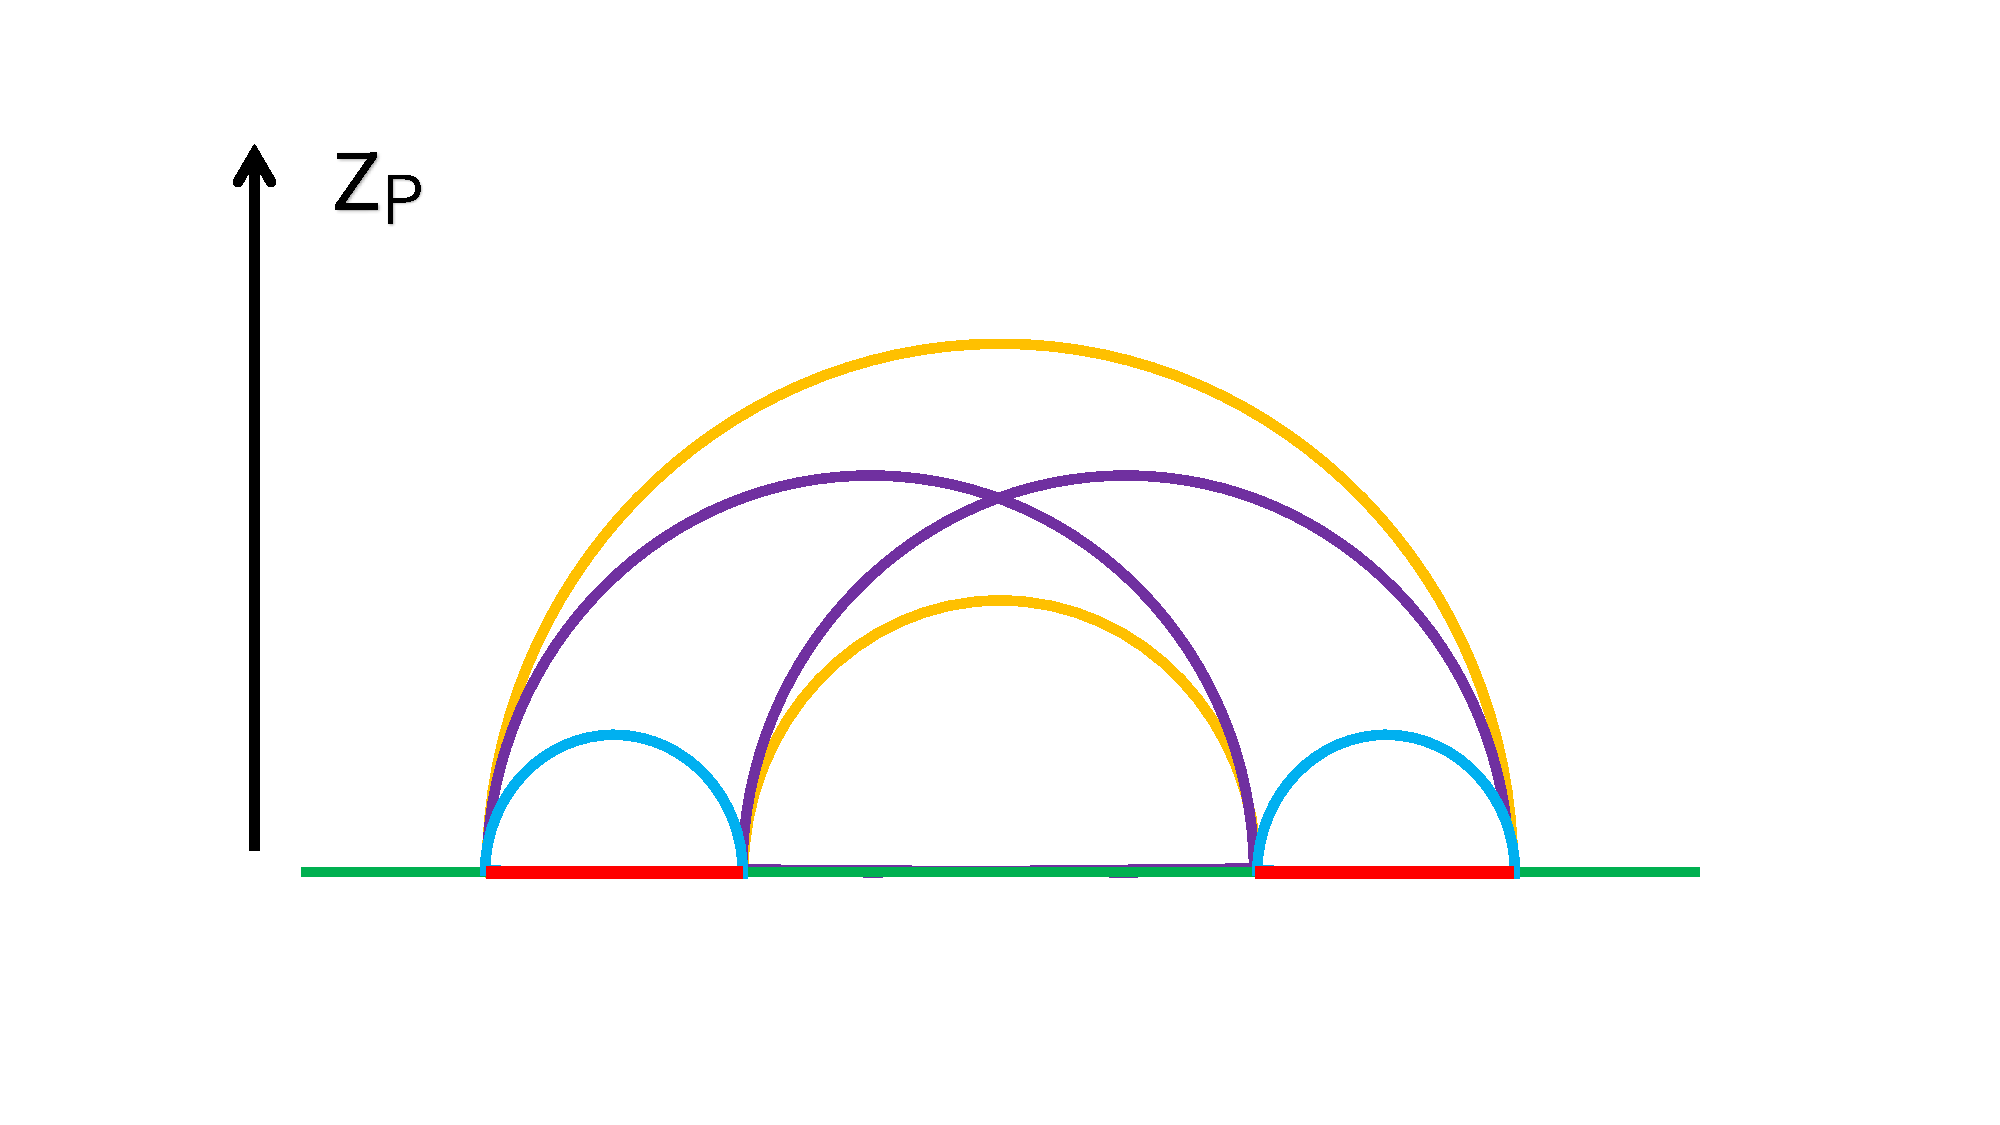
\includegraphics[width=0.7\linewidth]{disconnRTsurface.pdf}
	\label{fig:disconnRTsurface}
	\caption{Poincare座標の境界に定義された、2次元共形場理論の部分系$N=2$の部分系(赤い部分)と、その境界から伸ばした測地線の図。オレンジ・紫・水色の3通りの伸ばし方が考えられる。}
\end{figure}

よって右辺は
\begin{align}
RHS&=\frac{R_A}{2G}\log \frac{\min \left\{ |x_1-x_2|||x_3-x_4|, |x_1-x_3|||x_2-x_4|, |x_1-x_4|||x_2-x_3| \right\}}{\epsilon^2}\\
&=\frac{R_A}{2G}\log \frac{\min \left\{ |x_1-x_2|||x_3-x_4|, |x_1-x_4|||x_2-x_3| \right\}}{\epsilon^2}
\end{align}
となる。したがってAdS$_3$/CFT$_2$対応から、この場合も確かに笠-高柳公式が成立することが分かる。

$|x_1-x_2|||x_3-x_4|$の測地線と非連結区間Aで作られるループは2つの連結成分をもち、この測地線はしばしば\textbf{disconnected geodesic}と呼ばれる。また、$|x_1-x_4|||x_2-x_3|$の測地線と非連結区間Aで作られるループは1つの連結成分をもち、この測地線はしばしば\textbf{connected geodesic}と呼ばれる。

また、$|x_1-x_3|||x_2-x_4|$の寄与が現れないことは、エンタングルメントエントロピーの強劣加法性に対応している。実際、強劣加法性(\ref{ssa})から左辺のエンタングルメントエントロピーに対して
\begin{align}
S(\rho_{[x_1,x_2]})+S(\rho_{[x_3,x_4]})\le S(\rho_{[x_1,x_3]})+S(\rho_{[x_2,x_4]})
\end{align}
が成り立つので、$|x_1-x_3|||x_2-x_4|$の寄与が現れることは無い。このことは右辺では$\min$をとる操作によって実現されている。

\subsub{具体例5 : 円筒上のCFTの低温状態での、連結区間Aのエンタングルメントエントロピー}
半径$L$の円筒上の温度$\beta\gg L$の低温状態$\rho=e^{-\beta H}$について、連結区間$A=[x_1,x_2]$に対して笠-高柳公式の両辺を計算する。

一般にトーラス2点関数の計算は、平面上の2点関数のように中心電荷のみでは決まらないが、$\beta\gg 1$の極限を考えると、
\begin{align}
LHS\sim \frac{c}{3}\log \left(\frac{2L}{\epsilon}\sin\left(\frac{x_1-x_2}{2L}\right)\right)
\end{align}
となる。これは真空の場合の結果に整合している。

この共形場理論に対応する時空は温度$\beta_A\gg 1$のthermal AdSであり、右辺は
\begin{align}
RHS=\frac{\text{length}(\gamma)}{4G}=\frac{R_A}{2G}\log \left(\frac{2L}{\epsilon}\sin\left(\frac{x_1-x_2}{2L}\right)\right)
\end{align}
となる。したがってAdS$_3$/CFT$_2$対応から、この場合も確かに笠-高柳公式が成立することが分かる。

\subsub{具体例6 : 円筒上のCFTの高温状態での、小さな連結区間Aのエンタングルメントエントロピー}
半径$L$の円筒上の温度$\beta\ll L$の高温状態$\rho=e^{-\beta H}$について、小さな連結区間$A=[x_1,x_2],\ |x_1-x_2|\ll L$に対して笠-高柳公式の両辺を計算する。この場合も平面上の有限温度状態の場合と同じで、
\begin{align}
LHS&=S(\rho_A)=\frac{c}{3}\log\left(\frac{2\beta}{\epsilon}\sinh\left(\frac{x_1-x_2}{2\beta}\right)\right)\\
RHS&=\frac{\text{length}(\gamma)}{4G}=\frac{R_A}{2G}\log \left(\frac{2\beta R_A^{-1}}{\epsilon'}\sinh\left(\frac{x_1-x_2}{2\beta R_A^{-1}}\right)\right)
\end{align}
となり、AdS$_3$/CFT$_2$対応から、この場合も確かに笠-高柳公式が成立することが分かる。

\subsub{具体例7: 円筒上のCFTの高温状態での、全体系のエントロピー}
半径$L$の円筒上の温度$\beta\ll L$の高温状態$\rho=e^{-\beta H}$について、全体系に対して笠-高柳公式の両辺を計算する。左辺は単にカノニカル分布$\rho=e^{-\beta H}$のvon Neumannエントロピーであり、$\beta\gg L$より(\ref{cardyCE})から
\begin{align}
LHS\sim \frac{c}{3}\pi \beta^{-1}
\end{align}
となる。また右辺のホモロジー条件を満たす最小測地線は、BTZブラックホールのホライズンを1周するような曲線であり、(\ref{btzwindingcurvelength})より、
\begin{align}
RHS=\frac{2\pi R_A^2\beta_A^{-1}}{4G}=\frac{c_A}{3}\pi R_A\beta_A^{-1}
\end{align}
となる。AdS$_3$/CFT$_2$対応から、この場合も確かに笠-高柳公式が成立することが分かる。また、このことは笠-高柳公式がBekenstein-Hawking公式の一般化になっていることを表す。

\subsection{HRT公式}
笠-高柳公式は、Euclid時間の理論に対する公式である。笠-高柳公式のLorentz時間への拡張は、Hubeny,Rangamani,高柳\cite{Hubeny:2007xt}によって提案されている。この提案は次のようなものである。

$A$が定義されているCFTの時刻$t=t_\ast$のCauchy面を境界に持つような重力側のCauchy面$\Sigma$をとるごとに、上の境界条件とホモロジー条件を満たす長さ最小の曲線$\gamma_\Sigma \of \Sigma$が決まり、$\gamma_\Sigma$の長さのうち最大のものが、エンタングルメントエントロピーを与える。
\begin{oframed}
\begin{align}
S_A(t_\ast)=\max_{\del\Sigma=(t=t_\ast\text{面})} \min_{\substack{\gamma_\Sigma\of\Sigma\\ \del\gamma_\Sigma=\del A\\ \gamma_\Sigma\text{と}A\text{で作られるループは0にホモロガス}}} \frac{\text{Area}(\gamma_\Sigma)}{4G_N}
\end{align}
\end{oframed}
